\documentclass{beamer}
\usepackage{amsmath,amssymb,latexsym,array,fancyheadings,mathdots}
\usepackage{algorithm,algorithmic}
\usepackage{hyperref}
\usepackage{color}
\usepackage{tabularx}
\usepackage[all]{xy}
\usepackage{qtree}
\usepackage{gitinfo2}

%% RCS
%\usepackage{rcs}

%% Colors
\definecolor{darkgreen}{rgb}{0,.4,0}
\definecolor{darkred}{rgb}{.5,0,0}
\definecolor{darkmagenta}{rgb}{.5,0,.5}
\definecolor{orange}{rgb}{1,.5,0}
\definecolor{lightblue}{rgb}{0.122,0.016,0.855}
\definecolor{darkocre}{rgb}{0.471,0.298,0.008}

\usetheme{default}

%% New Theorems
\newtheorem{thm}{Theorem}
\newtheorem{exm}[thm]{Example}
\newtheorem{cor}[thm]{Corollary}
\newtheorem{propo}[thm]{Proposition}
\newtheorem{lem}[thm]{Lemma}
\newtheorem{clm}[thm]{Claim}
\newtheorem{exr}[thm]{Exercise}
\newtheorem{dfn}[thm]{Definition}

%% New commands
\newcommand{\classfont}{\mathsf}
\newcommand{\ATM}{\classfont{A}_{\mathrm{TM}}}
\newcommand{\MTF}{\mathrm{MTF}}
\newcommand{\OPT}{\mathrm{OPT}}
\newcommand{\ALG}{\mathrm{ALG}}
\newcommand{\ALGNAIVE}{\mathrm{ALG}_{\text{na{\"\i}ve}}}
\newcommand{\LRU}{\mathrm{LRU}}
\newcommand{\FIFO}{\mathrm{FIFO}}
\newcommand{\FWF}{\mathrm{FWF}}
\newcommand{\LFD}{\mathrm{LFD}}
\newcommand{\true}{\mathsf{T}}
\newcommand{\false}{\mathsf{F}}
\newcommand{\also}{\wedge}
\newcommand{\lra}{\leftrightarrow}
\newcommand{\tc}{\textcolor}
\newcommand{\df}[1]{\textcolor{red}{\em #1}}
\newcommand{\highlight}[1]{\textcolor{orange}{\em #1}}
\newcommand{\hl}[1]{\textcolor{blue}{\em #1}}
\newcommand{\amp}{\texttt{\&}}
\newcommand{\hsh}{\texttt{\#}}
\newcommand{\ra}{\rightarrow}
\newcommand{\longra}{\longrightarrow}
\newcommand{\Ra}{\Rightarrow}
\newcommand{\rab}{{\rightarrow_\beta}}
\newcommand{\srab}{{\rightarrow^*_\beta}}
\newcommand{\aeq}{{=_\alpha}}
\newcommand{\order}{\mathrm{order}}
\newcommand{\rem}{\mathrm{rem}}
\newcommand{\IP}{\mathbf{IP}}
\newcommand{\PSPACE}{\mathbf{PSPACE}}
\newcommand{\thevalue}{\text{value}}
\newcommand{\pol}[1]{\mathbf{#1}}
\newcommand{\enc}{\text{Enc}}
\newcommand{\xor}{\oplus}
\newcommand{\zo}{\{0,1\}}
\newcommand{\SOPT}{S_{\mathrm{opt}}}
\newcommand{\la}{\leftarrow}
\newcommand{\myurl}[1]{\textcolor{darkgreen}{\url{#1}}}
\newcommand{\myhref}[2]{\textcolor{darkgreen}{\href{#1}{#2}}}
\newcommand{\qaccept}{q_{\mathrm{accept}}}
\newcommand{\qreject}{q_{\mathrm{reject}}}
\newcommand{\opt}{\text{\sc Opt}}
\newcommand{\tr}{\mathrm{tr}}
\newcommand{\csanky}{p^{\textsc{csanky}}}
\newcommand{\berk}{p^{\textsc{berk}}}

%% Algorithms package customization
\renewcommand{\algorithmicrequire}{\textbf{Pre-condition:}} 
\renewcommand{\algorithmicensure}{\textbf{Post-condition:}} 
\algsetup{indent=3em}

\input{prooftree}

%% including/excluding pauses
\newcommand{\ifpause}{\iftrue} % for including pauses
%\newcommand{\ifpause}{\iffalse} % for excluding pauses

%% 2nd or 3rd edition
\newif\ifthird
\thirdtrue
%\thirdfalse

%disables usefoottemplate
\setbeamertemplate{navigation symbols}{}
%\setbeamertemplate{footline}% 
%{\strut\quad\tiny 
%\begin{minipage}{3cm}
%Cryptography - Michael Soltys
%\today\ {\tt v\RCSRevision}
%\end{minipage}\hfill
%\insertsection\
%- \insertframenumber/\inserttotalframenumber\quad\strut}

\newcommand{\mytitle}{Computational Foundations \\ Section 9.4}
\newcommand{\mychpnr}{9}
%% Title page contents
\title{Intro to Analysis of Algorithms \\ \mytitle \\  Chapter \mychpnr}
\author{Michael Soltys}
\date{\textcolor{darkgreen}{\tiny\tt 
[ {\bf Git} Date:\gitAuthorDate\ 
Hash:\gitAbbrevHash\ 
Ed:\ifthird
3rd
\else
2nd
\fi]}}
\institute{CSU Channel Islands}

\setbeamertemplate{footline}{
  \colorbox{white}{\color{black}\tt
     \begin{tabularx}{0.97\textwidth}{XXX}
          IAA Chp \mychpnr\ - Michael Soltys \copyright & 
          \hfill\today\ (\gitAbbrevHash; \ifthird ed3\else ed2\fi)
					\hfill\phantom{.} & 
          \hfill\insertsection\ - \insertframenumber/\inserttotalframenumber \\
      \end{tabularx}}}

\begin{document}

\mode<presentation>
{
}

\parskip 8pt

\section{Introduction}

\begin{frame}
\titlepage
\end{frame}


\begin{frame}
\begin{center}
\addtocounter{part}{1}
{\bf Part \Roman{part} \\ Context-free languages}
\end{center}
\end{frame}

\begin{frame}
A \df{context-free grammar (CFG)} is $G=(V,T,P,S)$
--- Variables, Terminals, Productions, Start variable

Ex. $P\longrightarrow\varepsilon|0|1|0P0|1P1$.

Ex. $G=(\{E,I\},T,P,E)$ where $T=\{+,*,(,),a,b,0,1\}$ and $P$ is the
following set of productions:
\begin{align*}
E & \longrightarrow I|E+E|E*E|(E) \\
I & \longrightarrow a|b|Ia|Ib|I0|I1
\end{align*}
If $\alpha A\beta\in(V\cup T)^*$, $A\in V$, and
$A\longrightarrow\gamma$ is a production, then $\alpha
A\beta\Rightarrow\alpha\gamma\beta$.  We use
$\stackrel{*}{\Rightarrow}$ to denote 0 or more steps.

$L(G)=\{w\in T^*|S\stackrel{*}{\Rightarrow}w\}$
\end{frame}

\begin{frame}

{\bf Lemma:}
$L((\{P\},\{0,1\},\{P\longrightarrow\varepsilon|0|1|0P0|1P1\},P))$ is
the set of palindromes over $\{0,1\}$.

{\bf Proof:} Suppose $w$ is a palindrome; show by induction on $|w|$
that $P\stackrel{*}{\Rightarrow}w$.

BS: $|w|\le 1$, so $w=\varepsilon,0,1$, so use
$P\longrightarrow\varepsilon,0,1$.  \\
IS: For $|w|\ge 2$, $w=0x0,1x1$, and
by IH $P\stackrel{*}{\Rightarrow}x$.

Suppose that $P\stackrel{*}{\Rightarrow}w$; show by induction on the
number of steps in the derivation that $w=w^R$.

BS: Derivation has 1 step. \\ 
IS: $P\Rightarrow 0P0\stackrel{*}{\Rightarrow}0x0=w$ (or with 1 instead of 0).
\end{frame}

\begin{frame}

If $S\stackrel{*}{\Rightarrow}\alpha$, then $\alpha\in (V\cup T)^*$,
and $\alpha$ is called a \df{sentential form}.  
$L(G)$ is the set of those
sentential forms which are in $T^*$.

Given $G=(V,T,P,S)$, the \df{parse tree} for $(G,w)$ is a tree with
$S$ at the root, the symbols of $w$ are the leaves (left to right),
and each interior node is of the form:
\begin{center}
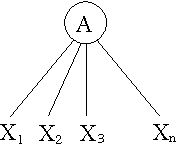
\includegraphics{figures/8.pdf}
\end{center}
whenever we have a rule $A\longrightarrow X_1X_2X_3\ldots X_n$
\end{frame}

\begin{frame}
Derivation: head $\longrightarrow$ body \\
Recursive Inference: body $\longrightarrow$ head

The following five are all equivalent:
\begin{enumerate}
\item  Recursive Inference
\item  Derivation
\item  Left-most derivation
\item  Right-most derivation
\item  Yield of a parse tree.
\end{enumerate}
\end{frame}

\begin{frame}

{\bf Ambiguity of Grammars}

$E\Rightarrow E+E\Rightarrow E+E*E$ \\
$E\Rightarrow E*E\Rightarrow E+E*E$

Two different parse trees!  Different meaning.

A grammar is ambiguous if there exists a string $w$ with two different
parse trees.
\end{frame}

\begin{frame}

A \df{Pushdown Automaton (PDA)} is an $\varepsilon$-NFA with a stack.

Two (equivalent) versions: (i) accept by final state, (ii) accept by
empty stack.

PDAs describe CFLs.

The PDA pushes and pops symbols on the stack; the stack is assumed to
be as big as necessary.

Ex.  What is a simple PDA for $\{ww^R|w\in\{0,1\}^*\}$ ?
\end{frame}

\begin{frame}
Formal definition of a PDA:

$P=(Q,\Sigma,\Gamma,\delta,q_0,Z_0,F)$

$Q$ finite set of states

$\Sigma$ finite input alphabet

$\Gamma$ finite stack alphabet, $\Sigma\subseteq\Gamma$

$\delta(q,a,X)=\{(p_1,\gamma_1),\ldots,(p_n,\gamma_n)\}$

if $\gamma=\varepsilon$, then the stack is popped, if $\gamma=X$, then
the stack is unchanged, if $\gamma=YZ$ then $X$ is replaced $Z$, and
$Y$ is pushed onto the stack

$q_0$ initial state

$Z_0$ start symbol

$F$ accepting states
\end{frame}

\begin{frame}

A \df{configuration} is a tuple $(q,w,\gamma)$:
state, remaining input, contents of the stack

If $(p,\alpha)\in\delta(q,a,X)$, then
$(q,aw,X\beta)\ra(p,w,\alpha\beta)$

{\bf Theorem:} If $(q,x,\alpha)\ra^*(p,y,\beta)$, then
$(q,xw,\alpha\gamma)\ra^*(p,yw,\beta\gamma)$

Acceptance by final state:
$L(P)=\{w|(q_0,w,Z_0)\ra^*(q,\varepsilon,\alpha),q\in F\}$

Acceptance by empty stack:
$L(P)=\{w|(q_0,w,Z_0)\ra^*(q,\varepsilon,\varepsilon)\}$

{\bf Theorem:} $L$ is accepted by PDA by final state iff it is
accepted by PDA by empty stack.

{\bf Proof:} When $Z_0$ is popped, enter an accepting state.  For the
other direction, when an accepting state is entered, pop all the
stack.
\end{frame}

\begin{frame}

{\bf Theorem:} CFGs and PDAs are equivalent.

{\bf Proof:} From Grammar to PDA:
A left sentential form is $\underbrace{x}_{\in T^*}
\overbrace{A\alpha}^{\text{tail}}$

The tail appears on the stack, and $x$ is the prefix of the input that
has been consumed so far.

Total input is $w=xy$, and hopefully
$A\alpha\stackrel{*}{\Rightarrow}y$.

Suppose PDA is in $(q,y,A\alpha)$.  It guesses
$A\longrightarrow\beta$, and enters $(q,y,\beta\gamma)$.

The initial segment of $\beta$, if it has any terminal symbols, they
are compared against the input and removed, until the first variable
of $\beta$ is exposed on top of the stack.

Accept by empty stack.
\end{frame}

\begin{frame}
Ex.  Consider $P\longrightarrow \varepsilon|0|1|0P0|1P1$

The PDA has transitions: \\
$\delta(q_0,\varepsilon,Z_0)=\{(q,PZ_0)\}$ \\
$\delta(q,\varepsilon,P)=\{(q,0P0),(q,0),(q,\varepsilon),(q,1P1),(q,1)\}$\\
$\delta(q,0,0)=\delta(q,1,1)=\{(q,\varepsilon)\}$ \\
$\delta(q,0,1)=\delta(q,1,0)=\emptyset$ \\
$\delta(q,\varepsilon,Z_0)=(q,\varepsilon)$

Consider:
$P\Rightarrow 1P1
\Rightarrow 10P01
\Rightarrow 100P001
\Rightarrow 100001$

\bigskip

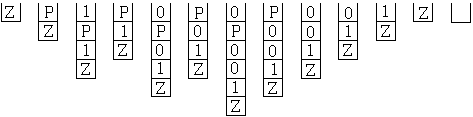
\includegraphics{figures/9.pdf}
\end{frame}

\begin{frame}
From PDA to grammar:

Idea: ``net popping'' of one symbol of the stack, while consuming some
input.

Variables: $A_{[pXq]}$, for $p,q\in Q$, $X\in\Gamma$.  

$A_{[pXq]}\stackrel{*}{\Rightarrow}w$ iff $w$ takes PDA from state $p$
to state $q$, and pops $X$ off the stack.

Productions: for all $p$, $S\longrightarrow A_{[q_0Z_0p]}$, and
whenever we have:
$$
(r,Y_1Y_2\ldots Y_k)\in\delta(q,a,X)
$$ 
$A_{[qXr_k]}\longrightarrow aA_{[rY_1r_1]}A_{[r_1Y_2r_2]}\ldots
A_{[r_{k-1}Y_kr_k]}$ \\
where $a\in\Sigma\cup\{\varepsilon\}$, $r_1,r_2,\ldots,r_k\in Q$ are
all possible lists of states.

If $(r,\varepsilon)\in\delta(q,a,X)$, then we have
$A_{[qXr]}\longrightarrow a$.

{\bf Claim:} $A_{[qXp]}\stackrel{*}{\Rightarrow} w \iff
(q,w,X)\ra^*(p,\varepsilon,\varepsilon)$.
\end{frame}

\begin{frame}
A PDA is deterministic if $|\delta(q,a,X)|\le 1$, and the second
condition is that if for some $a\in\Sigma$ $|\delta(q,a,X)|=1$, then
$|\delta(q,\varepsilon,X)|=0$.

{\bf Theorem:} If $L$ is regular, then $L=L(P)$ for some deterministic
PDA $P$.

{\bf Proof:} ignore the stack.

DPDAs that accept by final state are {\bf not} equivalent to DPDAs
that accept by empty stack.
\end{frame}

\begin{frame}
$L$ has the \df{prefix property} if there exists a pair $(x,y)$,
$x,y\in L$, such that $y=xz$ for some $z$.

Ex. $\{0\}^*$ has the prefix property.

{\bf Theorem:}  $L$ is accepted by a DPDA by empty stack $\iff$ $L$ is
accepted by a DPDA by final state {\bf and} $L$ does not have the
prefix property.

{\bf Theorem:}  If $L$ is accepted by a DPDA, then $L$ is unambiguous.
\end{frame}

\begin{frame}
Eliminating useless symbols from CFG:

$X\in V\cup T$ is \df{useful} if there exists a derivation such that
$S\stackrel{*}{\Rightarrow}\alpha X\beta\stackrel{*}{\Rightarrow}w\in
T^*$ 

$X$ is \df{generating} if $X\stackrel{*}{\Rightarrow}w\in T^*$

$X$ is \df{reachable} if there exists a derivation
$S\stackrel{*}{\Rightarrow}\alpha X\beta$

A symbol is useful if it is generating and reachable.

Generating symbols:
Every symbol in $T$ is generating, and if $A\longrightarrow\alpha$ is
a production, and every symbol in $\alpha$ is generating (or
$\alpha=\varepsilon$) then $A$ is also generating.

Reachable symbols:
$S$ is reachable, and if $A$ is reachable, and
$A\longrightarrow\alpha$ is a production, then every symbol in
$\alpha$ is reachable.
\end{frame}

\begin{frame}
If $L$ has a CFG, then $L-\{\varepsilon\}$ has a CFG without
productions of the form $A\longrightarrow\varepsilon$

A variable is \df{nullable} if
$A\stackrel{*}{\Rightarrow}\varepsilon$

To compute nullable variables: if $A\longrightarrow\varepsilon$ is a
production, then $A$ is nullable, if $B\longrightarrow C_1C_2\ldots
C_k$ is a production and all the $C_i$'s are nullable, then so is $B$.

Once we have all the nullable variables, we eliminate
$\varepsilon$-productions as follows: eliminate all
$A\longrightarrow\varepsilon$.

If $A\longrightarrow X_1X_2\ldots X_k$ is a production, and $m\le k$
of the $X_i$'s are nullable, then add the $2^m$ versions of the rule
the the nullable variables present/absent (if $m=k$, do not add the
case where they are {\em all} absent).
\end{frame}

\begin{frame}
Eliminating unit productions:
$A\longrightarrow B$ \\
If $A\stackrel{*}{\Rightarrow}B$, then $(A,B)$ is a unit pair.

Find all unit pairs: $(A,A)$ is a unit pair, and if $(A,B)$ is a unit
pair, and $B\longrightarrow C$ is a production, then $(A,C)$ is a unit
pair.

To eliminate unit productions: compute all unit pairs, and if $(A,B)$
is a unit pair and $B\longrightarrow\alpha$ is a non-unit production,
add the production $A\longrightarrow\alpha$.  Throw out
all the unit productions.

A CFG is in \df{Chomsky Normal Form} if all the rules are of the form
$A\longrightarrow BC$ and $A\longrightarrow a$.

{\bf Theorem:}  Every CFL without $\varepsilon$ has a CFG in CNF.

{\bf Proof:} Eliminate $\varepsilon$-productions, unit
productions, useless symbols.  Arrange all bodies of
length $\ge 2$ to consist of only variables (by introducing new
variables), and finally break bodies of length $\ge 3$ into a cascade
of productions, each with a body of length exactly 2.
\end{frame}

\begin{frame}

{\bf Pumping Lemma for CFLs:} There exists a $p$ so that any $s$,
$|s|\geq p$, can be written as $s=uvxyz$, and:
\begin{enumerate}
\item  $uv^ixy^iz$ is in the language, for all $i\geq 0$,
\item  $|vy|>0$,
\item  $|vxy|\le p$
\end{enumerate}

Proof:
\begin{center}
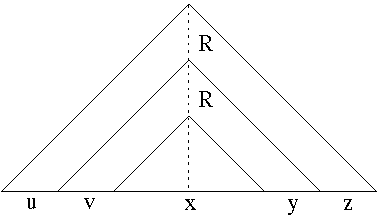
\includegraphics{figures/10.pdf}
\end{center}
\end{frame}

\begin{frame}
Ex. The lang $\{0^n1^n2^n|n\ge 1\}$ is not CF.

So CFL are not closed under intersection:
$L_1=\{0^n1^n2^i|n,i\ge 1\}$ and 
$L_2=\{0^i1^n2^n|n,i\ge 1\}$ are CF, but $L_1\cap L_2=\{0^n1^n2^n|n\ge
1\}$ is not.

{\bf Theorem:} If $L$ is a CFL, and $R$ is a regular language, then
$L\cap R$ is a CFL.

\end{frame}

\begin{frame}[fragile]

%Solution to 5.1.1c in Sipser
$L=\{ww:w\in\{0,1\}^*\}$ is not CF, but $L^c$ is CF.  So CFLs are not
close under complementation either.

We design a CFG for $L^c$.  First note that no odd strings are of the
form $ww$, so the first rule should be:
\begin{align*}
& S\longrightarrow O|E \\
& O\longrightarrow a|b|aaO|abO|baO|bbO
\end{align*}
here $O$ generates all the odd strings.  

$E$ generates
even length strings not of the form $ww$, i.e., all strings of the
form:
\begin{verbatim}
X=|_____0__|_____1__|  or  Y=|_____1__|_____0__|
\end{verbatim}
\end{frame}

\begin{frame}
We need the rule:
$$
E\longrightarrow X|Y
$$
and now
$$
\begin{array}{ll}
X\longrightarrow PQ   &  Y\longrightarrow VW  \\
P\longrightarrow RPR  &  V\longrightarrow SVS \\
P\longrightarrow a    &  V\longrightarrow b   \\
Q\longrightarrow RQR  &  W\longrightarrow SWS \\
Q\longrightarrow b    &  W\longrightarrow a   \\
R\longrightarrow a|b  &  S\longrightarrow a|b
\end{array}
$$

Ex.
\begin{align*}
X &\Ra PQ\Ra RPRQ\Ra RRPRRQ\Ra RRRPRRRQ\Ra RRRRPRRRRQ \\
  &\Ra RRRRRPRRRRRQ \Ra RRRRRaRRRRRQ\Ra RRRRRaRRRRRRQR \\
  &\Ra RRRRRaRRRRRRRQRR \Ra RRRRRaRRRRRRRbRR
\end{align*}
and now the R's can be replaced at will by a's and b's.
\end{frame}

\begin{frame}
CFL are closed under substitution: for every $a\in\Sigma$ we choose
$L_a$, which we call $s(a)$.  For any $w\in\Sigma^*$, $s(w)$ is the
language of $x_1x_2\ldots x_n$, $x_i\in s(a_i)$.

{\bf Theorem:} If $L$ is a CFL, and $s(a)$ is a CFL $\forall
a\in\Sigma$, then $s(L)=\cup_{w\in L}s(w)$ is also CF.

{\bf Proof:}
\begin{center}
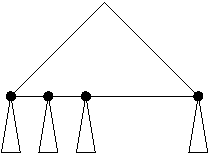
\includegraphics[width=3cm]{figures/11.pdf}
\end{center}

CFL are closed under union, concatenation, $*$ and $+$, homomorphism
(just define $s(a)=\{h(a)\}$, so $h(L)=s(L)$), and reversal (just
replace each $A\longrightarrow\alpha$ by $A\longrightarrow\alpha^R$).
\end{frame}

\begin{frame}
We can test for emptiness: just check whether $S$ is generating.
Test for membership: use CNF of the CYK algorithm (more efficient).

However, there are many {\bf undecidable} properties of CFL:
\begin{enumerate}
\item  Is a given CFG $G$ ambiguous?
\item  Is a given CFL inherently ambiguous?
\item  Is the intersection of two CFL empty?
\item  Given $G_1,G_2$, is $L(G_1)=L(G_2)$?
\item  Is a given CFL everything?
\end{enumerate}
\end{frame}

\begin{frame}
CYK\footnote{Cocke-Kasami-Younger} alg: 
Given $G$ in CNF, and $w=a_1a_2\ldots a_n$,
build an $n\times n$ table.
$w\in L(G)$ if $S\in (1,n)$.  ($X\in(i,j)\iff
X\stackrel{*}{\Rightarrow}a_ia_{i+1}\ldots a_j$.)

Let $V=\{X_1,X_2,\ldots,X_m\}$.  Initialize $T$ as follows:
\begin{tabular}{ll}
for & $(i=1; i\le n; i++)$ \\
    & for $(j=1; j\le m; j++)$
       Put $X_j$ in $(i,i)$ iff $\exists X_j\longrightarrow a_i$
\end{tabular}
Then, for $i<j$:
\begin{tabular}{ll}
for & $(k=i; k<j; k++)$ \\
    & if $(\exists\quad X_p\in (i,k)$ \&\ $X_q\in (k+1,j)$ 
       \&\ $X_r\longrightarrow X_pX_q)$ \\
    & Put $X_r$ in $(i,j)$
\end{tabular}
\footnotesize{%
\begin{tabular}[t]{|p{7mm}|p{7mm}|p{7mm}|p{7mm}|p{7mm}|}\hline
&&&& \\\hline
x&\textcolor{red}{(2,2)}&\textcolor{green}{(2,3)}
&\textcolor{blue}{(2,4)}&{\bf (2,5)} \\\hline
x&x&&&\textcolor{red}{(3,5)} \\\hline
x&x&x&&\textcolor{green}{(4,5)} \\\hline
x&x&x&x&\textcolor{blue}{(5,5)} \\\hline
\end{tabular}}
\end{frame}

\begin{frame}
\df{Context-sensitive grammars (CSG)} have rules of the form:
$$
\alpha\ra\beta
$$
where $\alpha,\beta\in(T\cup V)^*$ and $|\alpha|\le|\beta|$.  A
language is \df{context sensitive} if it has a CSG.

{\bf Fact:}  It turns out that $\text{CSL}=\text{NTIME}(n)$

A \df{rewriting system} (also called a \df{Semi-Thue system}) is a
grammar where there are no restrictions; $\alpha\ra\beta$ for
arbitrary $\alpha,\beta\in(V\cup T)^*$.  

{\bf Fact:}  It turns out that a rewriting system corresponds to the
most general model of computation; i.e., a language has a rewriting
system iff it is ``computable.''

Enter Turing machines $\ldots$
\end{frame}

\begin{frame}

{\bf Chomsky-Schutzenberger Theorem:} If $L$ is a CFL, then there
exists a regular language $R$, an $n$, and a homomorphism $h$, such
that $L=h(\text{PAREN}_n\cap R)$. 

{\bf Parikh's Theorem:} If $\Sigma=\{a_1,a_2,\ldots,a_n\}$, the
signature of a string $x\in\Sigma^*$ is $(\texttt{\#}a_1(x),
\texttt{\#}a_2(x),\ldots,\texttt{\#}a_n(x))$, i.e., the number of
ocurrences of each symbol, in a fixed order.  The signature of a
language is defined by extension; regular and CFLs have the same
signatures.
\end{frame}

\begin{frame}
\begin{minipage}{1.5cm}

\includegraphics[width=1.5cm]{figures/kozen.jpg}
\end{minipage}
\begin{minipage}{6cm}
Automata and Computability \\
Dexter Kozen
\end{minipage}

\begin{minipage}{1.5cm}

\includegraphics[width=1.5cm]{figures/sipser.jpg}
\end{minipage}
\begin{minipage}{6cm}
Intro to the theory of Computation \\
Third edition \\
Michael Sipser
\end{minipage}

\begin{minipage}{1.5cm}
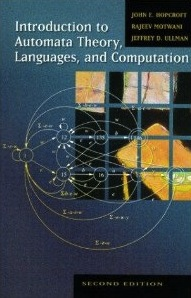
\includegraphics[width=1.5cm]{figures/hopcroft.jpg}
\end{minipage}
\begin{minipage}{9cm}
Intro to automata theory, languages and computation \\
Second edition \\
John Hopcroft, Rajeev Motwani, Jeffrey Ullman \\
{\em There is now a 3rd edition!}
\end{minipage}
\end{frame}

\end{document}
